\subsection{Application of Array in Image Analysis}
\subsubsection{Intensity Profile and Array Functions}

To learn the actual use of array in image analysis, we explore several example applications. In the first application, we use \ilcom{getProfile} function. We already used \ilcom{getProfile()} in the section \ref{subsec:numericalarray} ``Numerical Array''. This time, we use it in combination with Array functions to get local minima along the intensity profile - just like finding downward peak positions. We use a sample image Tree\textunderscore Rings.jpg (\ijmenu{[File > Open Samples > Tree Rings]}). 
 
We draw a straight line ROI crossing tree rings, and then the aim of the macro we will write is to detect ring positions along that line ROI and indicate those positions by point ROIs. The macro first reads the line-profile from the straight line ROI and then we use \ilcom{Array.findMinima} function to detect local minima (dark rings). Since this function returns the position of minima only as indices of the line-profile array, we need to get \ilcom{x} and \ilcom{y} coordinates of minima from their indices in order to plot minima positions in the original image. For this purpose, we resample the straight line ROI to the same number of points as the length of line-profile array. Let's write the code and learn by doing. 

Note: Before running the macro code20\_4.ijm, be sure to have a straight line ROI placed crossing tree rings (fig. \ref{fig:treeRingsSelected}). 

\begin{figure}[h!]
\begin{center}
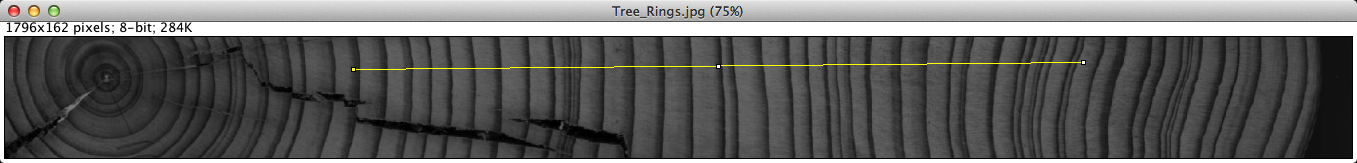
\includegraphics[width=0.9\textwidth]{fig/Tree_Rings_Selected.png}
\caption{A strainght Line ROI crossing rings.}
\label{fig:treeRingsSelected}
\end{center}
\end{figure}


\lstinputlisting[morekeywords={*, getProfile, Array, findMinima, resample, print, getStatistics}]{code/code20_4.ijm}


\begin{itemize}
\item line 3 - 4:  Check if the selection type is a straight line ROI using function \ilcom{selectionType}. If not, macro terminates leaving a message.
\item Line 5: An intensity profile array \ilcom{pA} is sampled by \ilcom{getProfile}().
\item Line 6: Detect local minima using \ilcom{Array.findMinima}. The first argument is the line-profile array, and the second argument is ``tolerance''. A larger tolerance value is less sensitive to intensity minimum - less detection. You could try changing this value later to see the effect. An array containing indices of minima positions is returned. 
\item Line 7: \ilcom{getSelectionCoordinates} with straight-line ROI stores two arrays, each for start/end x coordinates and start/end y coordinates. Two arrays, in this case \ilcom{xpoints} and \ilcom{ypoints}, have length of two. 
\item Line 8 - 9: Resampling of straight-line ROI by number of points in the line-profile array \ilcom{pA}.
\item Line 10-11: Prepare two new arrays to store x and y coordinates of minima positions. 
\item Line 12: For-loop to go through minima indices array. 
\item Line 13-14: \ilcom{minsA[i]} is the index for a single minimum, and using that index, x and y coordinate of that minimum position is retrieved and stored into new arrays prepared in line 10-11. 
\item Line 16: After the looping, x and y coordinates of minima are used in \ilcom{makeSelection} function to create multiple point ROI. 
\end{itemize}

Run the code, then you should see multiple point ROIs indicating positions of rings (See fig. \ref{fig:treeRingsSelected}). Similar macro can be used to measure striated pattens in tissues or cell edges. In case of fluorescence images, \ilcom{Array.findMaxima} can be used to detect high-intensity maxima positions. 

\begin{figure}[h!]
\begin{center}
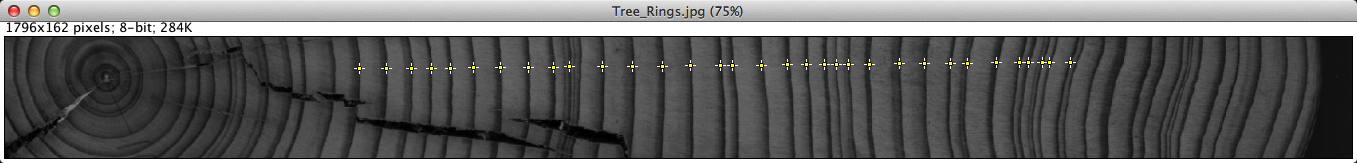
\includegraphics[width=0.9\textwidth]{fig/Tree_Rings_Minima.png}
\caption{Detected ring positions.}
\label{fig:treeRingsMinima}
\end{center}
\end{figure}


%\begin{indentexercise}{1}
%\item Add some codes that the macro also prints out the total intensity along the segment ROI. Use looping. \\
%\end{indentexercise}

\subsubsection{Extending Stack Analysis by Direct Measurements}

We studied how to use for-loops to measure each frame/slice within a stack (\ref{sec:forloopStack}). There we did measurements by firstly setting measurement parameters with \ilcom{run("Set Measurements...")} and then did measurement by \ilcom{run("Measure")}. Measured values were shown in the table in the ``Results'' window. To use those measured values to \textit{e.g.} calculate statistics or plot the results, one should access the table in the ``Results'' window and parse all the values. This is possible with the macro language, but we will not try this method as it is indirect. Instead, we try to access directly to the measured values and compute. There are two ways. 

\begin{enumerate}
\item \ilcom{getRawStatistics(nPixels, mean, min, max, std, histogram)}
\item \ilcom{List.setMeasurement}
\end{enumerate}
The function \ilcom{getRawStatistics} measures statistical parameters from the image and returns those values in the variables declared as arguments. In other words, after this function is executed, variable \ilcom{mean} will have the mean intensity of the image
\footnote{In this example we use a variable named \ilcom{mean}, but the name could be anything such as \ilcom{a} or \ilcom{b}.}. 
If a ROI is selected, mean intensity of that ROI will be the value of \ilcom{mean}. We could loop each slice/frame within a stack and for each loop we could do \ilcom{getRawStatistics} and store measured values in arrays. But there is a drawback of using this function: the available parameters to measure is limited. 

The second method \ilcom{List.setMeasurement} does not have this limitation. One could measure many more parameters because all the available parameters listed in \ilcom{[Analyze > Set Measurements...]} are accessible with this function. The basic usage is shown in the code below, which measures the currently active image, extracts specific measurement value (in this example case ``Mean'' intensity) and then prints out that value in the log window. Try writing this code and test it with any image. 

\begin{lstlisting}
List.setMeasurements;
mean = List.getValue("Mean");
print(mean)
\end{lstlisting}

We could do the measurement using \ilcom{List.setMeasurement} function for every loop for stack slices/frames and store the results in arrays. Here is the code, a modified version of code 10 (p~\pageref{code:10}). 

\lstinputlisting[morekeywords={*, List, setMeasurements, getValue, newArray}]{code/code10_1.ijm}

\begin{itemize}
  \item Line 2: Checks the ImageJ version, since \ilcom{List.setMeasurements} function is only available after version 1.42i.
  \item Line 5, 6: Create new arrays with their length equal to the number of frames of the stack. These arrays will be used to store measurement results. 
  \item Line7: for-loop going through each frames in the stack.
  \item Line 10: Measure. All the parameters will be stored in the List. 
  \item Line 11, 12: Retrieve the results, mean intensity and its standard deviation. 
  \item Line 15, 16: Print out results in the log window. 
\end{itemize}
